\documentclass[convert={density=100,outext=.png}]{standalone}
\usepackage{tikz}
\usetikzlibrary{arrows,patterns}

% defining the new dimensions and parameters
\newlength{\hatchspread}
\newlength{\hatchthickness}
\newlength{\hatchshift}
\newcommand{\hatchcolor}{}
\tikzset{hatchspread/.code={\setlength{\hatchspread}{#1}},
         hatchthickness/.code={\setlength{\hatchthickness}{#1}},
         hatchshift/.code={\setlength{\hatchshift}{#1}},% must be >= 0
         hatchcolor/.code={\renewcommand{\hatchcolor}{#1}}}
\tikzset{hatchspread=3pt,
         hatchthickness=0.4pt,
         hatchshift=0pt,% must be >= 0
         hatchcolor=black}
\pgfdeclarepatternformonly[\hatchspread,\hatchthickness,\hatchshift,\hatchcolor]% variables
   {custom north west lines}% name
   {\pgfqpoint{\dimexpr-2\hatchthickness}{\dimexpr-2\hatchthickness}}% lower left corner
   {\pgfqpoint{\dimexpr\hatchspread+2\hatchthickness}{\dimexpr\hatchspread+2\hatchthickness}}% upper right corner
   {\pgfqpoint{\dimexpr\hatchspread}{\dimexpr\hatchspread}}% tile size
   {% shape description
    \pgfsetlinewidth{\hatchthickness}
    \pgfpathmoveto{\pgfqpoint{0pt}{\dimexpr\hatchspread+\hatchshift}}
    \pgfpathlineto{\pgfqpoint{\dimexpr\hatchspread+0.15pt+\hatchshift}{-0.15pt}}
    \ifdim \hatchshift > 0pt
      \pgfpathmoveto{\pgfqpoint{0pt}{\hatchshift}}
      \pgfpathlineto{\pgfqpoint{\dimexpr0.15pt+\hatchshift}{-0.15pt}}
    \fi
    \pgfsetstrokecolor{\hatchcolor}
\pgfusepath{stroke}
   }
\begin{document}
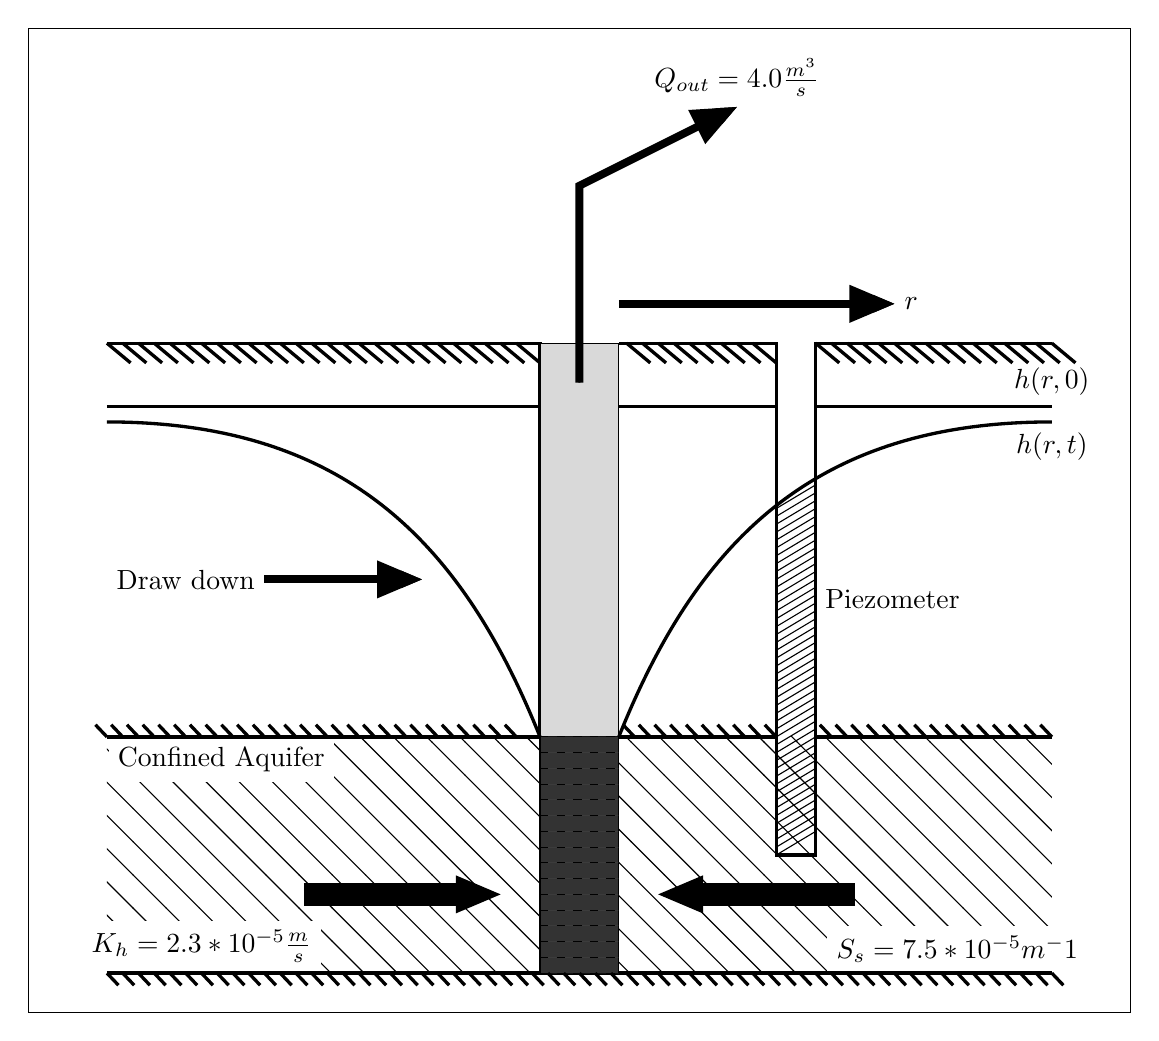
\begin{tikzpicture}
\tikzstyle{myarrows}=[line width=1mm,-triangle 45,postaction={draw, line width=3mm, shorten >=4mm, -}]
\tikzstyle{normarrow}=[line width=.25mm,-triangle 45,postaction={draw, line width=1mm }]
	\draw[fill=white] (-7,-8.5) rectangle (7,4);
	%Draws the top of the subsurface i.e. above the confined aquifer
	\draw[draw = none, pattern = custom north west lines,hatchspread=12pt] (-6,-8) rectangle (.5,-5);
	\draw[draw=none,pattern=custom north west lines,hatchspread=12pt] (6,-8) rectangle (.5,-5);
	\draw (-6,0) -- (-.5,0) -- (-.5,-5) -- (-6,-5)   [very thick] node[fill=white,anchor=north west] {Confined Aquifer};
	\draw (6,0) -- (3,0) -- node[pos =.5,right] {Piezometer}(3,-6.5) -- (2.5,-6.5) -- (2.5,0) -- (.5,0) [very thick] ;
	\draw (.5,-5) -- (2.5,-5) [very thick];
	\draw (3,-5) -- (6,-5) [very thick];

	%Draws the bottom of the confined aquifer
	\draw (-6,-8) -- (6,-8) [very thick] node[pos= 0.1 ,above,fill=white] {$K_h=2.3*10^{-5} \frac{m}{s}$} node[pos= .9 ,above,fill=white] {$S_s=7.5 *10^{-5} m^-1$};
	\foreach \x in {-6,-5.8,...,-0.7}
		\draw [very thick] (\x,0) -- (\x+0.3,-.25);
	\foreach \x in {6,5.8,...,3,2.2,2,...,.5}
		\draw [very thick] (\x,0) -- (\x+0.3,-.25);

	%Draws the area of the well directly above the confined aquifer
	\filldraw[fill=gray!30] (-.5,0) rectangle (.5,-5);
	
	\foreach \x in {-6,-5.8,...,-.8}
		\draw [very thick] (\x, -5,0) -- (-.3+\x,-5,-0.4pt);

	\foreach \x in {6,5.8,...,3.2,2.5,2.3,...,.6}
		\draw[very thick] (\x,-5,0) -- (-.3+\x,-5,-.4pt);

	%Draws the well directly in the confined aquifer
	\filldraw[fill=black!80] (-.5,-5) rectangle (.5,-8);
	
	\foreach \y in {-8,-7.8,...,-5}	
		\draw[style=dashed, fill=gray] 
			(-.5,\y) -- (.5,\y);

	\foreach \x in {-6,-5.8,...,6}
		\draw[very thick] (\x,-8,0) -- (\x+.3,-8,.4pt);
       
	%Draws the piezometer lines
	\foreach \y in {-6.5,-6.4,...,-2}
		\draw[fill =white,pattern =custom north west lines] (2.5,\y) -- (3,.3+\y);

	%Draws the draw down curve experienced in the confined aquifer and initial head
	\draw[very thick] (-.5,-5) .. controls (-1.5,-2.5) and (-3,-1) .. (-6,-1);
	\draw[very thick] (.5,-5) .. controls (1.5,-2.5) and (3,-1) .. (6,-1) node[anchor=north] {$h(r,t)$};
	\draw[very thick] (-6,-.8)--(-.5,-.8); 
	\draw [very thick](.5,-.8) -- (2.5,-.8);
	\draw [very thick] (3,-.8) -- (6,-.8) node[anchor=south] {$h(r,0)$};
        \draw [normarrow] (-4,-3) -- (-2,-3);
        \draw (-5,-3) node {Draw down}; 

	%Attributes of the confined aquifer (arrow and fill pattern)
	\draw[myarrows] (-3.5,-7)--(-1,-7) ;
	\draw[myarrows] (3.5,-7.0)--(1,-7) ;

	%Define Parameters
	\draw[normarrow] (0,-.5)-- (0,2)--(2,3) node[anchor=south] {$Q_{out} = 4.0 \frac{m^3}{s}$};
	\draw [normarrow] (.5,.5) -- (4,.5) node [anchor=west] {$r$};
	
\end{tikzpicture}

\end{document}